\section{Introduction}
\label{sec:introduction}

% state the learning objective 
The objective of this laboratory assignment is to study a given circuit, described in the figure~\ref{fig:circuito} below, running a theoretical analysis as well as a simulation and compare both of the results.

\begin{figure}[H] \centering
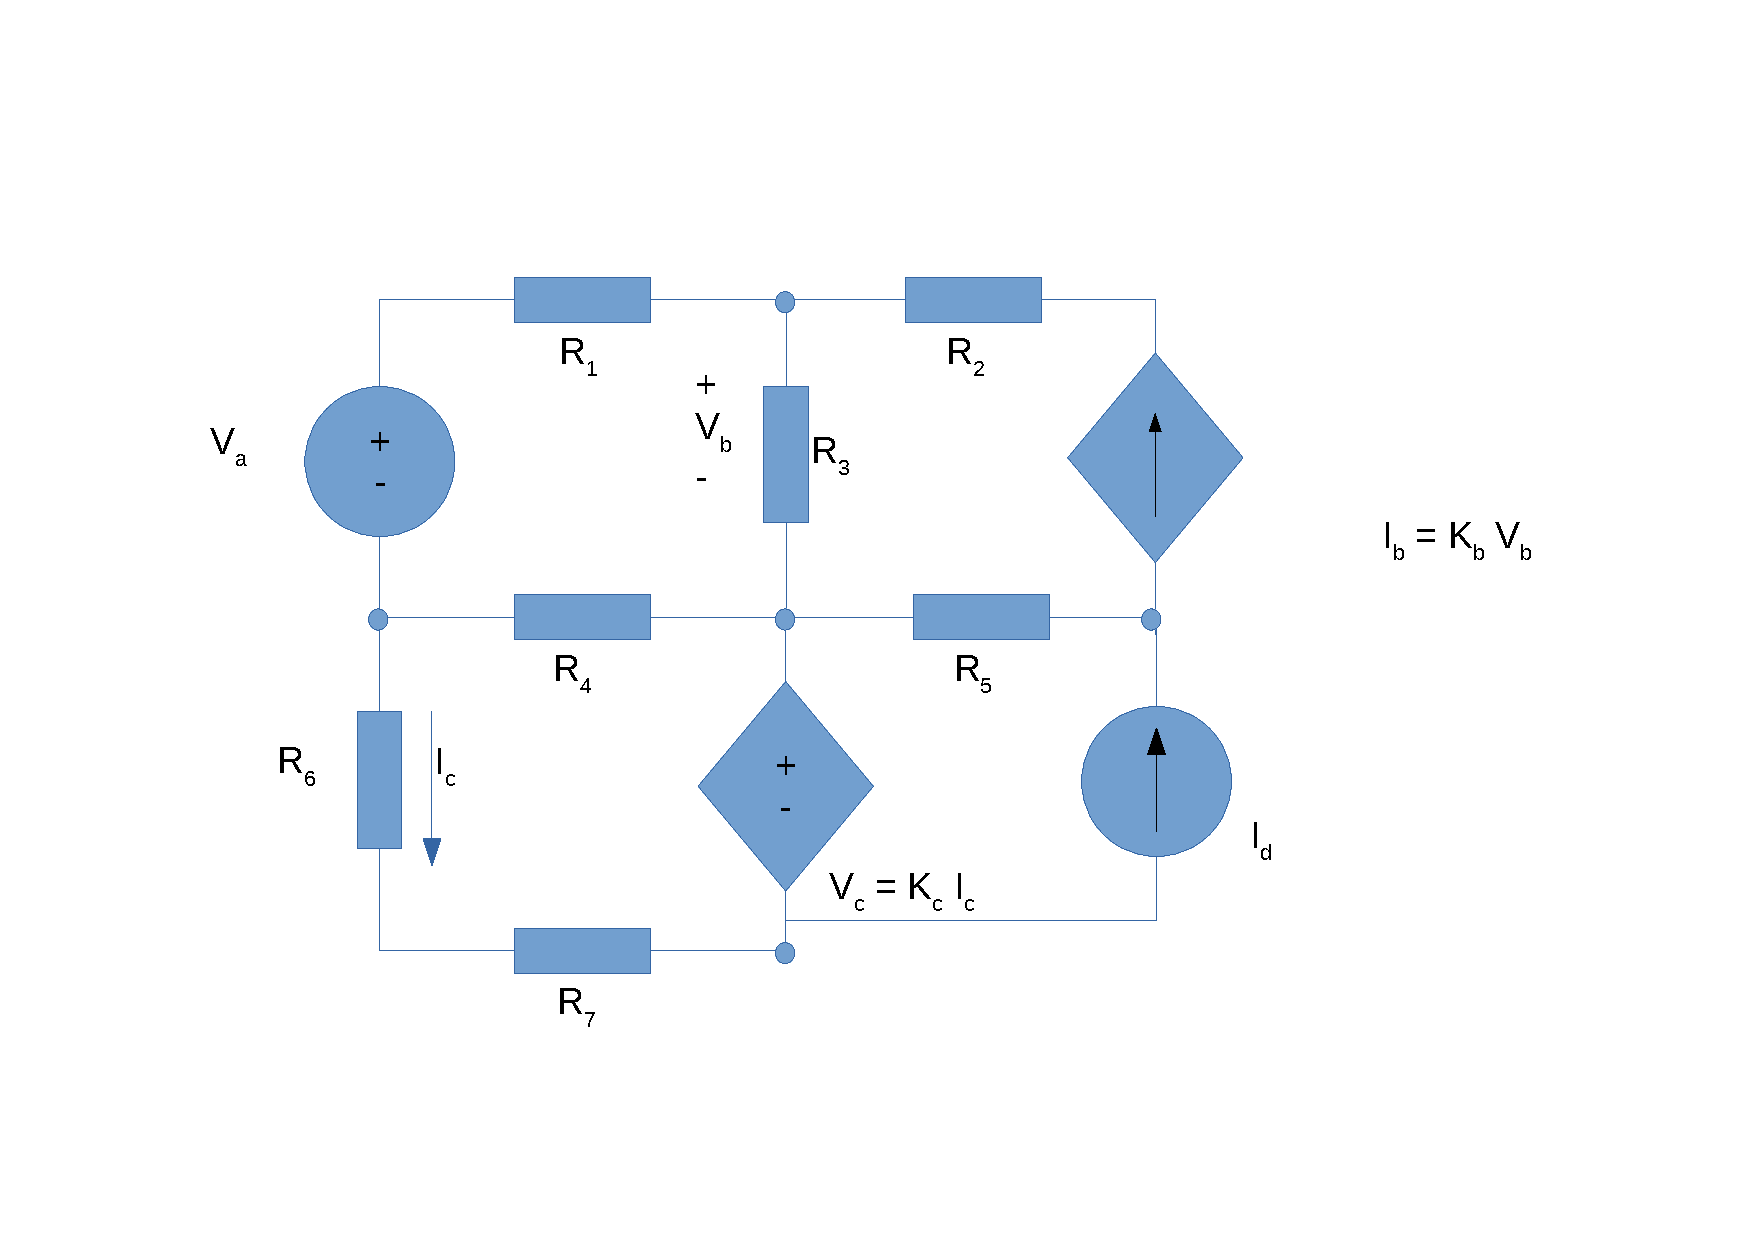
\includegraphics[width=0.7\linewidth]{circuito.pdf}
\caption{T1's given circuit.}
\label{fig:circuito}
\end{figure}

The theoretical analysis will be done using both the mesh method as well as the nodal method. For the simulation, it will be done using a simple script on Ngspice. \par
The comparison between the three results will be made in the "Analysis" section of this report, where we will explain the small differences that we may get in our results.


